\section{INTO-CPS Method Guidelines}
\label{sec:method}

\subsection{Introduction}
\label{sec:method:intro}

The INTO-CPS tool chain enables collaborative multidisciplinary model-based design of CPSs. Although each discipline involved in a CPS engineering enterprise has its own culture, abstractions, and approaches to problem solving, it may only be on federating them that knowledge which is otherwise tacit in some disciplines has to be made explicit. To date, there is only limited experience in model-based multidisciplinary design of CPSs, and so the methods and approaches for bringing models together are only beginning to emerge. This section aims to distil the methods and guidelines that have emerged in our experience with the INTO-CPS toolchain, and to do so in a way that helps the reader understand how best to use INTO-CPS co-modelling technologies.

This section complements the Tool Chain User Manual~\cite{INTOCPSD4.3a}--- which gives detail on how to use the features of the tool chain--- by providing guidance on when and why you might use these features. The guidance given here has been distilled from experience gained through pilot studies and applications of INTO-CPS technologies to real industrial cases. These pilot studies now appear as examples that can be opened directly from the INTO-CPS Application, supported by descriptions in the Examples Compendium~\cite{INTOCPSD3.6}. Industrial applications are described in the Case Studies report~\cite{INTOCPSD1.3a}. Sections~\ref{sec:method:intro}--\ref{sec:method:workflows} provide an introduction to core INTO-CPS terminology and the activities that INTO-CPS enables. Advanced topics including traceability, design space exploration, architectural modelling, New users are recommended to:

%\begin{itemize}[noitemsep]
\begin{itemize}
  \item Read the introductory material in Sections~\ref{sec:method:intro}--\ref{sec:method:workflows}.
  \item Follow the first tutorial to experience the INTO-CPS Application.
  \item Import one or two examples from the Examples Compendium\footnote{\url{https://github.com/INTO-CPS-Association/training/tree/master/tutorials}} into the INTO-CPS Application and interact with them.
  \item As you start your own multi-modelling, return to this section for guidance on particular topics as required.
\end{itemize}

\subsection{Concepts and Terminology}
\label{sec:method:concepts}

Given the diversity of backgrounds in CPS engineering teams, it is worth clarifying some common concepts.

\subsubsection{Systems}
\label{sec:concepts:systems}
A \term{System} is ``a combination of interacting elements organized to achieve one or more stated purposes''~\cite{INCOSEseh15}. Any given system will have an~\term{environment}, considered to be everything outside of the system. The behaviour exhibited by the environment is beyond the direct control of the developer~\cite{Broenink&12b}. A \term{system boundary} is the common frontier between a system of interest and its environment~\cite{Broenink&12b}. An \term{interface} is a shared boundary between two entities, which can be defined in terms of physical and digital interactions and flows~\cite{INCOSEseh15}.


\term{Cyber-Physical Systems (CPSs)} are ``ICT systems (sensing, actuating, computing, communication, etc.) embedded in physical objects, interconnected (including through the Internet) and providing citizens and businesses with a wide range of innovative applications and services''~\cite{Thompson13, Deka&15}.

Many CPSs are \term{Systems of Systems (SoSs)}. An SoS is a ``collection of independent systems, integrated into a larger system that delivers unique capabilities''~\cite{INCOSEsosprimer18}.
%Many CPSs are \term{Systems of Systems (SoSs)}. An SoS is a ``collection of constituent systems that pool their resources and capabilities together to create a new, more complex system which offers more functionality and performance than simply the sum of the constituent systems''~\cite{Holt&14}. CPSs may exhibit the characteristics of SoSs.

\subsubsection{Models}
\label{sec:concepts:models}

A \term{model} is a  potentially partial and abstract description of a system, limited to those components and properties of the system that pertain to the current goal~\cite{Holt&14}. A model should be ``just complex enough to describe or study the phenomena that are relevant for our problem context''~\cite{Amerongen10}. Models should be abstract ``in the sense that aspects of the product not relevant to the analysis in hand are not included''~\cite{Fitzgerald&98b}. A model ``may contain representations of the system, environment and stimuli''~\cite{Fitzgerald&14c}

%\fbox{Further discussion may be required on the definition of: environment models, test models in RT-Tester and their correspondence in the INTO-CPS SysML profile?}.

In a CPS model, we describe systems with cyber, physical and network elements. These components are often modelled in a variety of languages, with different notations, concepts, levels of abstraction, and semantics, which are not necessarily easily mapped one to another. We use \term{continuous time (CT)} and \term{discrete event (DE)} models to represent physical and cyber elements as appropriate. A CT model has state that can be changed and observed \emph{continuously}~\cite{Amerongen10} and is described using either explicit continuous functions of time or implicitly as a solution of differential equations. A DE model has state that can be changed and observed only at fixed, \emph{discrete}, time intervals~\cite{Amerongen10}.  We use the term \term{multi-model} to refer to the federation of several constituent DE and CT models.

A \term{requirement} may impose restrictions, define capabilities or identify qualities of a system, and should indicate some value or use for the stakeholders in a CPS. \term{Requirements Engineering (RE)} is the process of specifying and documenting requirements placed upon a CPS. Requirements may be considered in relation to different \term{contexts} -- that is the point of view of some system component or domain, or interested stakeholder.

A \term{design parameter} is a property of a model that can be used to affect the model's behaviour, but remains constant during a given simulation~\cite{Broenink&12b}. A \term{variable} is feature of a model that may change during a given simulation~\cite{Broenink&12b}. \term{Non-functional properties (NFPs)} pertain to characteristics other than functional correctness. For example, reliability, availability, safety and performance of specific functions or services are NFPs that are quantifiable. Other NFPs may be more difficult to measure~\cite{Payne&10}.

The activity of creating models may be referred to as \term{modelling} ~\cite{Fitzgerald&14c} and related terms include \term{co-modelling} and \term{multi-modelling}. A \term{workflow} is a sequence of \term{activities} performed to aid in modelling. A workflow has a defined purpose, and may cover a subset of the CPS engineering development lifecycle.

The term \term{architecture} has many different definitions, and range in scope depending upon the scale of the product being `architected'. We use the simple definition from~\cite{COMPASSD22.6}:  ``an architecture defines the major elements of a system, identifies the relationships and interactions between the elements and takes into account process. Those elements are referred to as \term{components}. An architecture involves both a definition of structure and behaviour. Importantly, architectures are not static but must evolve over time to reflect the change in a system as it evolves to meet changes to its requirements''. In a CPS architecture, components may be either \term{cyber components} or \term{physical components} is they describe computational or physical elements.

We consider both \term{holistic} and a \term{design} architectures~(Section~\ref{sec:method:sysml}). The aim of a holistic architecture is to identify the units of functionality of the system reflecting the \emph{terminology and structure of the domain of application}. It describes a conceptual model of these units and their interconnections, giving a holistic view of the overall system. The design architectural model of the system is effectively a multi-model. The INTO-CPS SysML profile~\cite{INTOCPSD2.1a} is designed to assist in the specification of CPS design architectures. It helps the architect describe a system as a decomposition into interconnected \term{subsystems}, each of which is an assembly of cyber and physical components and possibly other subsystems. Each of these components and subsystems can be modelled separately in a domain-specific notation and tool.

\term{Evolution} refers to the ability of a system to benefit from a varying number of alternative system components and relations, as well as its ability to gain from the adjustments of the individual components' capabilities over time.
%An \term{interface} defines the boundary across which two entities meet and communicate with each other~\cite{Holt&14}. Interfaces may describe both digital and physical interactions: digital interfaces  contain descriptions of operations and attributes that are \emph{provided} and \emph{required} by components. Physical interfaces describe the flow of physical matter (for example fluid and electrical power) between components.

There are many methods of describing architectures. An \term{architecture diagram} is a symbolic representation of architectural information contained in a model. An \term{architectural framework} is a ``defined set of viewpoints and an ontology'' and ``is used to structure an architecture from the point of view of a specific industry, stakeholder role set, or organisation. In the application of an architecture framework, an \term{architectural view} is a ``work product (for example an architecture diagram) expressing the architecture of a system from the perspective of specific system concerns''~\cite{COMPASSD22.6}.

The \into\ SysML profile comprises diagrams for architectural modelling and specifying \term{design space exploration}. There are two architectural diagrams. The \term{Architecture Structure Diagram (ASD)} specialises SysML block definition diagrams to support the specification of a system architecture described in terms of a system's components. \term{Connections Diagrams (CDs)} specialise SysML internal block diagrams to convey the internal configuration of the system's components and the way they are connected. The system architecture defined in the profile should inform a co-simulation multi-model and therefore all components interact through connections between flow ports. The profile permits the specification of \term{cyber} and \term{physical} components and also components representing the \term{environment} and \term{visualisation} elements. The \into\ SysML profile includes three design space exploration diagrams: a \term{parameters diagram}; an \term{objective diagram}; and a \term{ranking diagram}. See Section~\ref{sec:concepts:analysis} for concepts relating to design space exploration.


\subsubsection{Tools}
\label{sec:concepts:tools}

The \term{\into\ tool chain} is a collection of software tools, based centrally around FMI-compatible co-simulation, that  supports the collaborative development of CPSs. The \term{\into\ Application} is a front-end to the INTO-CPS tool chain. The Application allows the specification of the co-simulation configuration, and the co-simulation execution itself. The application also provides access to features of the tool chain without an existing user interface (such as design space exploration and model checking).

Central to the \into\ tool chain is the use of the \term{Functional Mockup Interface (FMI)} standard. This is a tool-independent standard to support both model exchange and co-simulation of dynamic models using a combination of XML-files and compiled C-code~\cite{FMIStandard2.0}. Part of the FMI standard for model exchange is specification of a \term{model description} file. This is an XML file that supplies a description of all properties of a model (for example input/output variables). A \term{Functional Mockup Unit (FMU)} is a tool component that implements FMI. Data exchange between FMUs and the synchronisation of all simulation solvers~\cite{FMIStandard2.0} is controlled by a \term{Master Algorithm}.

\term{Co-simulation}  is the simultaneous, collaborative, execution of models and allowing information to be shared between them. The models may be CT-only, DE-only or a combination of both. The \term{Co-simulation Orchestration Engine (COE)} combines existing co-simulation solutions (FMUs) and scales them to the CPS level, allowing CPS multi-models to be evaluated through co-simulation. This means that the COE implements a \term{Master Algorithm}. The COE will also allow real software and physical elements to participate in co-simulation alongside models, enabling both Hardware-in-the-Loop (HiL) and Software-in-the-Loop (SiL) simulation.

In the \into\ Application, a \term{project} comprises: a number of FMUs, optional source models (from which FMUs are exported); a collection of \term{multi-models}; and an optional SysML architectural model. A multi-model includes a list of FMUs, defined instances of those FMUs, specified connections between the inputs/outputs of the FMU instances, and defined values for design parameters of the FMU instances. For each multi-model a \term{co-simulation configuration} defines the step size configuration, start and end time for the co-simulation of that multi-model. Several configurations can be defined for each multi-model.

\term{Code generation} is the transformation of a model into generated code suitable for compilation into one or more target languages (e.g. C or Java).

We consider two tool-supported methods for recording the rationale of design decisions in CPSs.  \term{Traceability} is the association of one model element (e.g., requirements, design artefacts, activities, software code or hardware) to another. \term{Requirements traceability} ``refers to the ability to describe and follow the life of a requirement, in both a forwards and backwards direction''~\cite{Gotel&94}. \term{Provenance} ``is information about entities, activities, and people involved in producing a piece of data or thing, which can be used to form assessments about its quality, reliability or trustworthiness'' ~\cite{Moreau&13}. In \into\ traceability between model elements defined in the various modelling tools is achieved through the use of \term{OSLC messages}, handled by a traceability \term{daemon tool}. This supports the \term{impact analysis} and general \term{traceability queries}.

Two broad groups of users are considered in the \into\ project. A \term{Tool Chain User} is an individual who uses the \into\ Tool Chain and its various analysis features. A \term{Foundations Developer} is someone who uses the developed foundations and associated tool support (see Section~\ref{sec:concepts:formal}) to reason about the development of tools.

\subsubsection{Analysis}
\label{sec:concepts:analysis}

\term{Design-Space Exploration (DSE)} is ``an activity undertaken by one or more engineers in which they build and evaluate [multi]-models in order to reach a design from a set of requirements''~\cite{Broenink&12b}. ``The \term{design space} is the set of possible solutions for a given design problem''~\cite{Broenink&12b}. Where two or more models represent different possible solutions to the same problem, these are considered to be \term{design alternatives}. In \into\, design alternatives are defined using either a range of parameter values or different multi-models. Each choice involves making a selection from alternatives on the basis of an \term{objective} -- criteria or constraints that are important to the developer, such as cost or performance. The alternative selected at each point constrains the range of design alternatives that may be viable next steps forward from the current position. Given a collection of alternatives with corresponding objective results, a \term{ranking} may be applied to determine the `best' design alternative.

\term{Test Automation (TA)} is defined as the machine assisted automation of system tests. In \into, we concentrate on various forms of \term{model-based testing} -- centering on testing system models, against the requirements on the system. The \term{System Under Test (SUT)} is ``the system currently being tested for correct behaviour. An alias for system of interest, from the point of view of the tester''~\cite{Holt&14}. The SUT is tested against a collection of \term{test cases} --  a finite structure of input and expected output~\cite{Utting&06}, alongside a \term{test model}, which specifies the expected behaviour of a system under test~\cite{Coleman&13b}. TA uses a \term{test suite} -- a collection of \term{test procedures}. These test procedures are detailed instructions for the set-up and execution of a given set of test cases, and instructions for the evaluation of results of executing the test cases~\cite{DO178B}.

\into\ considers three main types of test automation: \term{Hardware-in-the-Loop (HiL)}, \term{Software-in-the-Loop (SiL)} and \term{Model-in-the-Loop (MiL)}. In \term{HiL} there is (target) hardware involved, thus the FMU is mainly a wrapper that interacts (timed) with this hardware; it is perceivable that realisation heavily depends on hardware interfaces and timing properties.
%testing with DE models running on target hardware components;
In \term{Software-in-the-Loop (SiL)} testing the object of the test execution is an FMU that contains a software implementation of (parts of) the system. It can be compiled and run on the same machine that the COE runs on and has no (defined) interaction other than the FMU-interface.
%    It does not matter (much) where this implementation comes from.
%testing with software running on CT model simulator;
Finally, in \term{Model-in-the-Loop (MiL)} the test object of the test execution is a (design) model, represented by one or more FMUs. This is similar to the SiL (if e.g., the SUT is generated from the design model), but MiL can also imply that running the SUT-FMU has a representation on model level; e.g., a playback functionality in the modelling tool could some day be used to visualise a test run.
%testing with co-simulated CT/DE models. \fbox{Check definitions}

\term{Model Checking (MC)} exhaustively checks whether the model of the system meets its specification~\cite{Clarke&99}, which is typically expressed in some temporal logic such as \term{Linear Time Logic (LTL)}~\cite{Pnueli77} or \term{Computation Tree Logic (CTL)}~\cite{Clarke&81}. As opposed to testing, model checking examines the entire state space of the system and is thus able to provide a correctness proof for the model with respect to its specification. In INTO-CPS, we can concentrate on \term{Bounded Model Checking (BMC)}~\cite{Clarke&01,Clarke&04,Clarke&05}, which is based on encodings of the system in propositional logic, for a timed variant of LTL. The key idea of this approach is to represent the semantics of the model as a Boolean formula and then apply a \term{Satisfiability Modulo Theory (SMT)}~\cite{Kroening&08} solver in order to check whether the model satisfies its specification. A powerful feature of model checking is that, if the specification is violated, it provides a counterexample trace that shows exactly how an undesired state of the system can be reached~\cite{Clarke&03}.

\subsubsection{Existing Tools and Languages}
\label{sec:concepts:language}

The \into\ tool chain uses several existing modelling tools. \term{Overture}\footnote{\url{http://overturetool.org/}} supports modelling and analysis in the design of discrete, typically, computer-based systems using the \term{VDM-RT} notation. VDM-RT is based upon the \term{object-oriented} paradigm where a model is comprised of one or more \term{objects}. An object is an instance of a \term{class} where a class gives a definition of zero or more \term{instance variables} and \term{operations} an object will contain. Instance variables define the identifiers and types of the data stored within an object, while operations define the behaviours of the object.

The \term{20-sim}\footnote{\url{http://www.20sim.com/}} tool can represent continuous time models in a number of ways. The core concept is that of connected \term{blocks}.   \term{Bond graphs} may implement blocks. Bond graphs offer a domain-independent description of a physical system's dynamics, realised as a directed graph. The vertices of these graphs are idealised descriptions of physical phenomena, with their edges (\term{bonds}) describing energy exchange between vertices. Blocks may have input and output \term{ports} that allow data to be passed between them. The energy exchanged in 20-sim is the product of \term{effort} and \term{flow}, which map to different concepts in different domains, for example voltage and current in the electrical domain.

\term{OpenModelica}\footnote{\url{https://www.openmodelica.org/}}  is an open-source \term{Modelica}-based modelling and simulation environment. Modelica is an ``object-oriented language for modelling of large, complex, and heterogeneous physical systems''~\cite{Fritzson&98}. Modelica models are described by \term{schematics}, also called \term{object diagrams}, which consist of connected components. Components are connected by ports and are defined by sub components or a textual description in the Modelica language.

\term{Modelio}\footnote{\url{http://www.modelio.org/}} is an open-source modelling environment supporting industry standards like UML and SysML. \into\ will make use of Modelio for high-level system architecture modelling using the \term{SysML} language and proposed extensions for CPS modelling. The systems modelling language (SysML)~\cite{SysML12}  extends a subset of the UML to support modelling of heterogeneous systems.

\subsubsection{Formalisms}
\label{sec:concepts:formal}

The \term{semantics} of a language describes the meaning of a (grammatically correct) program~\cite{Nielson&92} (or model). There are different methods of defining a language semantics: \term{structural operational semantics}; \term{denotational semantics}; and \term{axiomatic semantics}.

A structural operational semantics (SOS) describes how the individual steps of a program are executed on an abstract machine~\cite{Plotkin81}. An SOS definition is akin to an interpreter in that it provides the meaning of the language in terms of relations between beginning and end states. The relations are defined on a per-construct basis. Accompanying the relations are a collection of semantic rules which describe how the end states are achieved. Where an operational semantics defines how a program is executed, a denotational approach defines a language in terms of denotations, in the form of abstract mathematical objects, which represent the semantic function that maps over the inputs and outputs of a program~\cite{Scott&71}.

The Unifying Theories of Programming (UTP)~\cite{Hoare&98} provides a unified framework for describing language semantics. A theory of a language is composed of an \term{alphabet}, a \term{signature} and a collection of \term{healthiness conditions}.

The Communicating Sequential Processes \term{CSP} notation~\cite{Hoare85} is a formal process algebra for describing  communication  and interaction.
\term{INTO-CSP} is a version of CSP, which will be used to provide a model for the SysML-FMI profile, FMI, VDM-RT and Modelica semantics. It is a front end for a UTP theory of reactive concurrent continuous systems customised for the needs of INTO-CPS. \term{Hybrid-CSP} is a continuous version of CSP defined originally by He Jifeng~\cite{Jifeng94}. It will be used as a basis to inform the design of INTO-CSP.

Several forms of verification are enabled through the use of formally defined languages.  \term{Refinement} is a verification and formal development technique pioneered by~\cite{Back&98} and~\cite{Morgan90a}. It is based on a behaviour preserving relation that allows the transformation of an abstract specification into more and more concrete models, potentially leading to an implementation. \term{Proof} is the process of showing how the validity of one statement is derived from others by applying justified rules of inference~\cite{Bicarregui&94}. For the purposes of verification in INTO-CPS, we make use of the Isabelle/HOL theorem prover and the FDR3 refinement checker. These are not considered part of the INTO-CPS tool chain, but were used in the INTO-CPS project primarily to support the development of foundation work.


\subsection{Activities Enabled by INTO-CPS}
\label{sec:method:workflows}
The following activities are all enabled by one or more of the INTO-CPS technologies. They are grouped into broad categories and include both existing, embedded systems activities and activities enabled by INTO-CPS, since INTO-CPS extends traditional embedded systems design capabilities towards CPS design. The choice of granularity for defining these activities naturally affects the size of such a list. The level chosen is instructive for describing workflows, but one that does not make the described workflows overly long.  %For example, those under the \textbf{Design} will often be supported by \textbf{Modelling} activities, but not necessarily.

In the following descriptions (and corresponding summary in Table~\ref{tab:activities}), we identify the tools that support the activities, where applicable, using the following icons:

\begin{itemize}[noitemsep]
\item[\INTOCPS] The INTO-CPS Application, COE and its extensions.
\item[\Modelio] Modelio.
\item[\Overture] The Overture tool.
%\item[\Crescendo] The Crescendo tool.
\item[\RTTester] RT-Tester.
\item[\OpenModelica] OpenModelica.
\item[\TwentySim] 20-sim.
\end{itemize}

Descriptions of these tools can be found in Section~\ref{sec:concepts:language}. Those activities in \emph{italics} can be recorded by the traceability features of INTO-CPS, which are described in Section~\ref{sec:method:trace}.

\newpage
\paragraph{Requirements and Traceability}

Writing \emph{Design Notes} (\INTOCPS) includes documentation about what has been done during a design, why a decision was made and so on. \emph{Requirements} (\Modelio) includes requirements gathering and analysis. \emph{Validation} (\INTOCPS) is any form of validation of a design or implementation against its required behaviour.

\paragraph{Architectural Modelling}

INTO-CPS primarily supports architectural modelling in SysML. \emph{Holistic Architectural Modelling} (\Modelio) and \emph{Design Architectural Modelling} (\Modelio) are described in Section~\ref{sec:method:sysml}. The former focuses on a domain-specific view, whereas the latter targets multi-modelling using a special SysML profile. The \emph{Export Model Descriptions} (\Modelio) activity indicated passing component descriptions from the Design Architectural Model to other modelling tools.

\paragraph{Modelling}

The \emph{Import Model Description} (\Overture~\TwentySim~\OpenModelica) activity means taking a component interface description from the Design Architectural Model into another modelling tool. \emph{Cyber Modelling} (\Overture) means capturing a ``cyber'' component of the system, e.g. using a formalism/tool such as VDM/Overture. \emph{Physical Modelling} (\TwentySim~\OpenModelica) means capturing the ``physical'' component of the system, e.g. in 20-sim  or OpenModelica. Collectively, these can be referred to as \emph{Simulation Modelling} (\Overture~\TwentySim~\OpenModelica) to distinguish from other forms, such as \emph{Architectural Modelling} (\Modelio). \emph{Co-modelling} (\Crescendo) means producing a system model with one DE and one CT part, e.g.\ in Crescendo. \emph{Multi-modelling} (\INTOCPS) means producing a system model with multiple DE or CT parts with several tools.

\paragraph{Design}

\emph{Supervisory Control Design} means designing some control logic that deals with high-level such as modal behaviour or error detection and recovery. \emph{Low Level Control Design} means designing control loops that control physical processes, e.g.\ PID control. \emph{Software Design} is the activity of designing any form of software (whether or not modelling is used). \emph{Hardware Design} means designing physical components (whether or not modelling is used).

\paragraph{Analysis}

In INTO-CPS, the RT-Tester tool enables the activities of \emph{Model Checking} (\RTTester), \emph{Creating Tests} (\RTTester) and creating a \emph{Test Oracle} (\RTTester) FMU. The \emph{Create a Configuration} (\INTOCPS) activity means preparing a multi-model for co-simulation. The \emph{Define Design Space Exploration Configurations} (\INTOCPS) activity means preparing a multi-model for multiple simulations. \emph{Export FMU} (\Overture~\TwentySim~\OpenModelica)  means to generate an FMU from a model of a component. \emph{Co-simulation} (\Crescendo~\INTOCPS) means simulating a co-model, e.g.\ using Crescendo baseline technology or the COE.

\paragraph{Prototyping}

\emph{Manual Code Writing} means creating code for some cyber component by hand. \emph{Generate Code} (\Overture~\TwentySim~\OpenModelica) means to automatically create code from a model of a cyber component. \emph{Hardware-in-the-Loop (HiL) Simulation} (\INTOCPS) and \emph{Software-in-the-Loop (HiL) Simulation} (\INTOCPS) mean simulating a multi-model with one or more of the models replaced by real code or hardware.

% The above activities are summarised in Table~\ref{tab:activities}. Terms in \emph{italics} correspond to INTO-CPS activities that produce traceable artifacts, as described in the traceability ontology in Deliverable D3.1b~\cite{INTOCPSD3.2b}.%\fbox{Are they there?}.

\begin{table}[p]
\centering
\caption{\protect{}Activities in existing embedded systems design workflows or enhanced INTO-CPS workflows.}\label{tab:activities}

% Entries in italics correspond to traceable artifacts in INTO-CPS (see Chapter~\ref{sec:trace})}

\begin{tabular}{ll}\hline
\multicolumn{2}{l}{\textbf{Requirements Engineering}} \\
{Stakeholder Documents} & \Modelio \\
Requirement Definition & \Modelio \\
Validation & \INTOCPS \\ \hline
\multicolumn{2}{l}{\textbf{Architectural Modelling}} \\
Holistic Architectural Modelling & \Modelio \\
Design Architectural Modelling & \Modelio \\
{Export Model Descriptions} & \Modelio \\ \hline
\multicolumn{2}{l}{\textbf{Modelling}} \\
{Import a Model Description} & \Overture~\TwentySim~\OpenModelica \\
Physical Modelling ({Simulation Modelling}) & \TwentySim~\OpenModelica \\
Cyber Modelling ({Simulation Modelling}) & \Overture \\
{Co-modelling} & \Crescendo \\
{Multi-modelling} & \INTOCPS \\ \hline
\multicolumn{2}{l}{\textbf{Design}} \\
Supervisory Controller Design & \\
Low Level Controller Design & \\
Software Design & \\
Hardware Design & \\ \hline
\multicolumn{2}{l}{\textbf{Analysis}} \\
{Create Tests} & \RTTester \\
{Model Checking} & \RTTester \\
{Create Test Oracle} & \RTTester \\
{Create a Configuration} & \INTOCPS \\
{Define Design Space Exploration Configurations} & \INTOCPS \\
{Export FMU} & \Overture~\TwentySim~\OpenModelica \\
Co-simulation  & \Crescendo~\INTOCPS \\ \hline
\multicolumn{2}{l}{\textbf{Prototyping}} \\
{Generate Code} & \Overture~\TwentySim~\OpenModelica \\
Hardware-in-the-Loop (HiL) Simulation & \INTOCPS \\
Software-in-the-Loop (SiL) Simulation & \INTOCPS \\
Manual Code Writing  & \\ \hline
\end{tabular}
\end{table}

\subsection{Configuring Multi-Models}

As discussed in Section~\ref{sec:method:concepts}, a multi-model  is a collection of FMUs with a configuration file that: defines instances of those FMUs, specifies connections between the inputs/outputs of the FMU instances, defines values for design parameters of the FMU instances, and defines other simulation settings such as a start, end time, and Master algorithm settings. As seen above, creating a multi-model is a key part of using the INTO-CPS tool chain as it is a pre-requisite for many of the analysis techniques that INTO-CPS can perform.

The INTO-CPS Application supports a project, a view of a folder containing source models, generated FMUs, and configuration files for co-simulation (multi-models) as well as configuration files for other analyses (design space exploration, model checking, test automation). Multi-model configurations can be created in three ways:

\begin{enumerate}[noitemsep]
  \item Created manually using the GUI of the INTO-CPS Application; or
  \item Generated from a SysML model created in Modelio; or
  \item Created manually by editing JSON configuration files
\end{enumerate}

All three approaches produce the same configuration file, so the choice of which to use depends on the engineer's background. Those comfortable with SysML may find it best to follow the SysML route, but this is not required. So those unfamiliar with SysML can use the Application directly.
These two approaches are covered in the second and third tutorials in Part~\ref{part:tutorials}. Manually editing the JSON configuration is an advanced topic that is not covered in the tutorials, but since JSON is human-readable, not complicated with some experimentation.

\subsection{First Steps for Users}
\label{sec:firststeps}
In this final section, we consider a how different types of users might approach the INTO-CPS technologies. As described in Section~\ref{sec:method:intro}, all new users are recommended to follow the first tutorial to experience the INTO-CPS Application, import one or two examples from the Examples Compendium (Deliverable D3.6~\cite{INTOCPSD3.6}) into the INTO-CPS Application and interact with them, returning to this section and Section~\ref{cha:advanced} as and when guidance on a particular area is required.


After initial familiarisation, the following list provides hints on next steps for different types of users, and where to find further information. As a reminder, updated tutorials supporting newer versions of the tool can be found at \url{https://github.com/INTO-CPS-Association/training/releases}.

% *****

\subsection{An Overview of Advanced Methods}
\label{cha:advanced}

\subsubsection{Traceability}
\label{sec:method:trace}

The technologies in the INTO-CPS tool chain are able to capture traceability information autonatically as activities are performed using the various elements of the tool chain. This includes information about who created or modified an artefact (model, simulation result etc.), and which requirements it is linked to. The traceability features of the INTO-CPS tool are described in depth in \cite{INTOCPSD3.3a}and the User Manual~\cite{INTOCPSD4.3a}.


The INTO-CPS tool chain builds a graph of traceability relations, as there can be multiple relationships between different artefacts. The graph is however tree-like in the sense that there must be some root node(s) to trace from or back to. These root nodes are \emph{requirements}. The traceability graph is initialised by using Modelio from the beginning of the development process. The traceability graph is then subsequently updated by the baseline tools as models are created from the model descriptions, FMUs are exported and so on, and co-simulation runs and results will be recorded by the INTO-CPS Application. By performing the required manual input of requirements and links to SysML elements, it is then possible to automatically trace forward to models, FMUs and simulation results, and to trace backwards from these artefacts to individual requirements.

Traceability in the tool chain is based upon a study of the actions performed when using the INTO-CPS tool chain, the artefacts that are used and produced and a combination of two existing standards, the W3C's Prov~\footnote{\url{https://www.w3.org/TR/prov-overview/}} and the OMG's OSLC~\footnote{\url{http://open-services.net/}}.   The combination of these resulted in the INTO-CPS traceability ontology that captures in detail all elements in the INTO-CPS workflow and describes the relationships between them.  The complete ontology is presented in~\cite{INTOCPSD3.3b}. Traceability data is inherently a graph based structure based upon nodes and the connections between them, and Prov provides basic types for those nodes along with list of relationships that may exist between them.  The three types of nodes are: Entities, things that may be produced or used during a development process; Activities, are things that act upon and make use of entities; and Agents, objects that have responsibility for entities and activities.  The Prov relations then allow then connection of nodes such as an activity may use an entity, and an entity may be generated by an activity.

The combination of the Prov nodes and relations supports the representation of the processes that lead to the generation of a particular entity, but it does not support connection of those entities to requirements.  OSLC contains a set of specifications, each of which defines a list of relations that it supports between entities. In the case of the INTO-CPS traceability, parts of the OSLC architecture management and requirements management specifications are employed, these allow the connection of entities to requirements via a 'satisfies' relation indicating the entity attempts to address the needs of the requirement, additionally it allows the connection of simulation results to requirements via a 'verifies' relation indicating that the requirement has been met.
Figure~\ref{fig:traceability:step02} shows the traceability links recorded during one step in the development of a line following robot.  In this example, the requirements, R1 \& R2, already exist in the architecture models and the user has created an ASD to decompose the proposed robot into components.  The user has, at the same time, associated the blocks within the ASD with the the requirements that each block aims to satisfy.  When the user saves the updates architecture model, the Modelio tool records the user's 'Architecture Modelling' activity, along with references to the ASD, the blocks it contains and the newly created links between the blocks and the requirements.  Here the \emph{used}, \emph{wgb} (short for 'was generated by'), \emph{assoc} (short for 'associated with') and \emph{attrib} (short for 'attributed to') are links that come from the Prov standard.  The \emph{OSLC\_Sat} (short for 'satisifies') comes from the OSLC requirements management specification.

%\draftnote{CJG: Give example of one action in detail}

\begin{figure}[htbp]
	\centering
	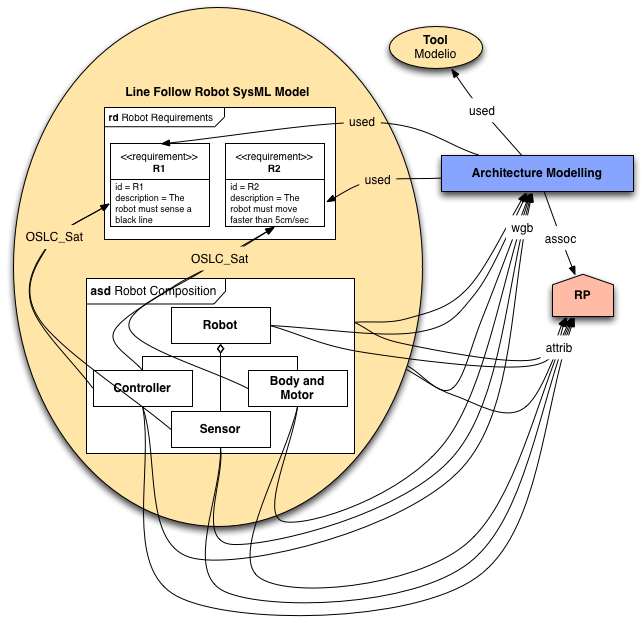
\includegraphics[width=0.8\textwidth]{figures/Traceability/step02}
\caption{Traceability links captured during the production of an ASD for a line following robot.}\label{fig:traceability:step02}
\end{figure}

%\draftnote{CJG: As the user(s) use the tools, they each record the their atomic actions, forming the traceability graph}

A development project will likely consist of many instances of the activities identified in the ontology being performed and together they form a traceability graph.  Figure~\ref{fig:traceability:abstractTraceFlow} shows a simplified view of a traceability graph with some steps removed for brevity.  At the top of the graph we see the architecture modelling step described previously, that produces an architecture model.  From the architecture, model description files are exported to start the production of the simulation models.  In turn the simulation models are exported as FMUs and the FMUs are used to produce simulation results.  Key to the traceability graph then are the 'used' and 'wgb' connections that can be used by a query to determine from where each entity was generated.  By following these links back from any entity to the individual blocks within the architecture model, it is possible to determine which requirement(s) each should satisfy.  Finally when simulation results are output, these may be linked back to the relevant requirements, stating whether a requirement was verified or violated by that result.

%\draftnote{CJG: Give abstract view of a resulting trace}


\begin{figure}[htbp]
	\centering
	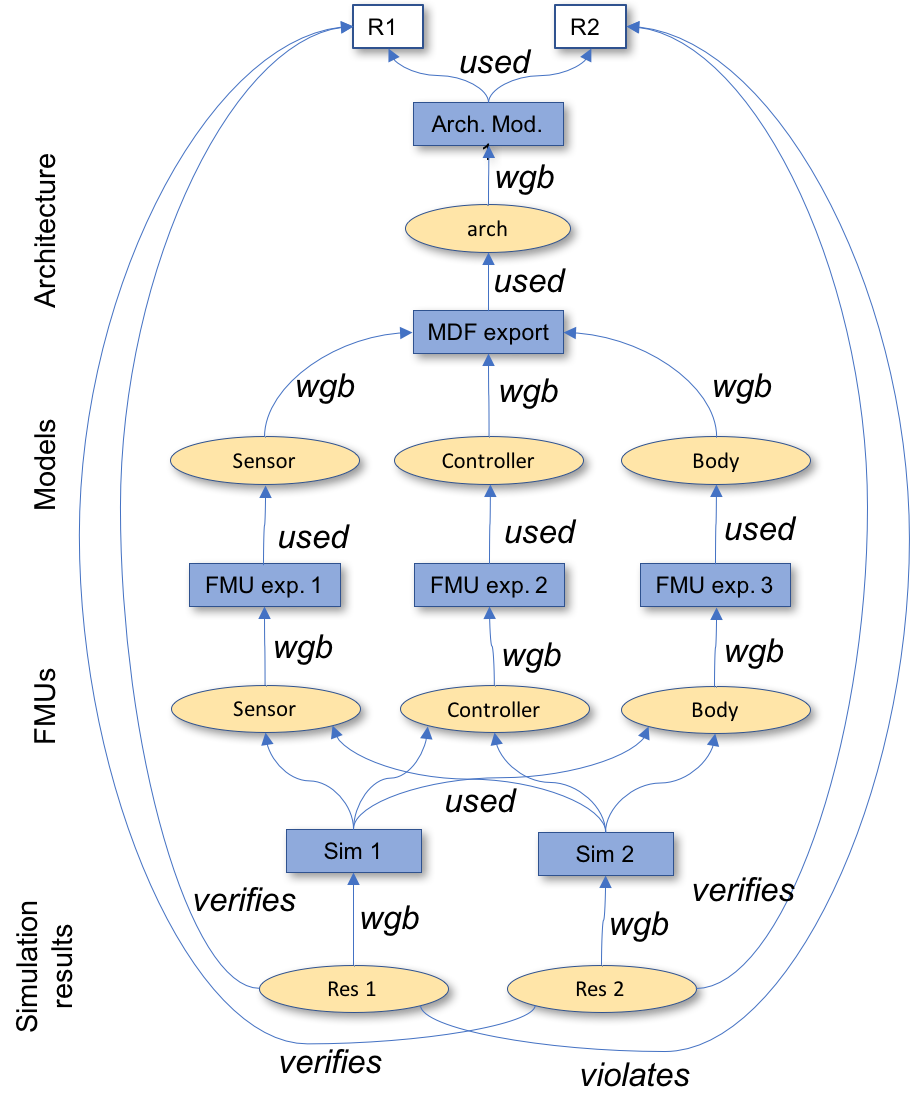
\includegraphics[width=0.7\textwidth]{figures/Traceability/abstractTraceFlow}
\caption{Traceability links captured during the production of an ASD for a line following robot.}\label{fig:traceability:abstractTraceFlow}
\end{figure}


%\draftnote{CJG: A paragraph outlining the entities, activities and agents}

The traceability ontology captures the significant activities and entities that form the INTO-CPS workflow.  For example a development project might see the following activities recorded in the traceability graph:  \emph{Requirements Management}, \emph{Architecture Modelling}, \emph{Architecture Configuration Creation} \emph{Model Description Export}, \emph{Simulation Modelling}, \emph{FMU Export}, \emph{Configuration Creation}, \emph{Simulation Configuration Creation} and then \emph{Simulation}.  These activities are connected in the workflow by the entities they create and use, so the example would see the traceability graph containing records of: \emph{Archtecture Structure Diagram}, \emph{Architecture SubSystem}, \emph{Architecture Connection Diagram}, \emph{Model Description File}, \emph{Simulation Model}, \emph{FMU}, \emph{Multi-model Configuration}, \emph{Simulation Configuration} and \emph{Simulation Result}.  Alongside these will be records of the agent(s), who are both associated with activities and have entities attributed to them.


Once a graph has been built, queries can be executed over the graph to perform both forwards and backwards traceability. Below are some types of queries that can be executed over the graphs. Examples include: forward traceability (from requirements to entities); backwards traceability (from FMU to requirements); finding sources and sinks for a simulation; assessing coverage such as finding requirements without positive simulation results; and evaluating user impact, such as finding all artefacts influenced by a given user.

\subsubsection{Requirements Engineering}
\label{sec:method:reqeng}

Requirements placed on a CPS may, for example, impose restrictions, define system capabilities or identify qualities of a system. The requirements should indicate some value or use for the different stakeholders of a CPS. Traceability needs requirements to be defined early in a development process, and these must be recorded in Modelio for the machine-assisted traceability information to be recorded accurately. It is therefore appropriate to consider requirements processes for such developments at this stage.

In the INTO-CPS Methods guidelines~\cite{INTOCPSD3.3b}, we describe one possible approach to RE for CPS, adapting an approach already piloted on tsystems-of-systems (SoSs). Note however that this approach is not mandatory, and in general RE processes and tools vary widely across organisations and domains. For this reason, tool support for traceability in INTO-CPS begins once requirements have been defined and can be added to Modelio. The approach was adapted from standard systems engineering, and tailored for SoSs--- enabling the identification and reasoning about requirements across constituent systems of an SoS and understanding multi-stakeholder contexts. We suggest it might be useful to organisations trying to approach RE for CPS.

In the approach, we propose a collection of views that could be represented as diagrams in SysML\footnote{Note that this approach is is not specifically supported as a Modelio plug-in, but other equivalent diagrams could be used.}, or could equally be represented in other tools where these are already used (e.g. Excel). Examples of views include:

\begin{description}
\item[Source Element View (SEV)] which defines a collection of source materials from which requirements are derived. This could be represented as a SysML block definition diagram ior an Excel table or Word document (with each source having a unique identifier), or by simply referring to source documents using OSLC traces.

\item[Requirement Description View (RDV)] which is used to define the requirements of a system and forms the core of the requirement definition. This can be done in a SysML requirements diagram or in tabulated form, such as through the use of Excel. In addition, specifying requirements in  Doors would support this view.

\item[Context Definition View (CDV)] The CDV is a useful view for CPS engineering in order to explicitly identify interested stakeholders and points of context in the system development, including customers, suppliers and system engineers themselves. In SoS-ACRE, they are defined using SysML block definition diagrams, and could also be represented using an Excel table or Word document (with each context having a unique identifier). This diagram type could be useful when identifying the divide in CT/DE and cyber-physical elements of a system.

\item[Requirement Context View (RCV)] In SoS-ACRE, a RCV is defined for each constituent system context identified in CDVs. This is appropriate when there is a set of diverse system owners, which is typical for SoSs and increasingly CPSs. A \textbf{Context Interaction View (CIV)} is then defined to understand the overlap of contexts and any common/conflicted views on requirements. In a CPS, however, there may not be such a clear delineation between the owners of constituent  system components. However, if we consider the different domains (e.g. CT/DE or cyber/physical divides) as different contexts, then this approach would be useful. In SoS-ACRE, RCVs and CIVs are both defined with SysML use case diagrams. Excel could be used if unique identifiers are defined for contexts and requirements as described earlier.

\item[Validation View (VV)] VVs, defined as SysML sequence diagrams in SoS-ACRE, describe validation scenarios for a SoS to ensure each constituent system context understands the correct role of the requirements in the full SoS. This is not an obvious fit in CPS engineering, and therefore not necessarily required.

\end{description}

The full RE process is described in greater detail in \cite{INTOCPSD3.3a} as a disciplined approach involving identifying and recording source elements (in an SEV), system-level functional and non-functional requirements (using RDVs), an initial system structure (in an INTO-CPS ASD, which identified cyber and physical elements), and relevant contexts in CDVs. Requirements may then be traced using INTO-CPS tool chain models and results.

\subsubsection{SysML and Multi-modelling}
\label{sec:method:sysml}

Standard SysML can be used as part of a development process to build a model of a system and link elements to requirements. The INTO-CPS tool chain also provides an extended SysML profile that help users to \emph{configure multi-models for co-simulation} and \emph{configure design space exploration (DSE) analysis}~\cite{INTOCPSD2.1a,INTOCPSD2.2a,INTOCPSD2.3a,INTOCPSD41c,INTOCPSD4.2c,INTOCPSD4.3c}.
The multi-modelling SysML profile defines two diagrams for configuring a co-simulation. The INTO-CPS Application can run a co-simulation based on a configuration file which describes the FMUs, their parameters and connections between them. There are two types diagram, the \emph{Architectural Structure Diagram (ASD)} describing the static structure of FMUs, and the \emph{Connections Diagram (CD)} describing their instantiation and connections. These are shown in Figure~\ref{fig:sysml:intocps}.

\begin{figure}[h!]
\centering
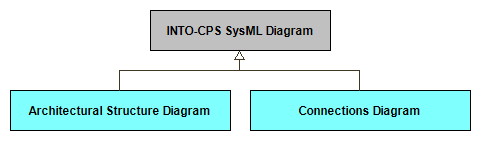
\includegraphics[scale=0.6]{figures/Architecting/ArchitecturalViews}
\caption{Diagrams in the multi-modelling SysML profile}
\label{fig:sysml:intocps}
\end{figure}

The design space exploration (DSE) SysML profile is an addition to the multi-modelling SysML profile described above. As with single co-simulation, the INTO-CPS Application can run a DSE based on a configuration file. Alternatively, a configuration can be generated by Modelio, from a set of diagrams defined in the profile. There are five diagram types (see Figure~\ref{fig:sysml:dse} which are used to define the objectives for a DSE and their instantiations, define the parameters that will be changed on each co-simulation in a DSE and their instantiations, and the objectives to be used for ranking competing designs.

\paragraph{Holistic and Design Architectural Modelling}
\label{sec:sysml:holistic}

A system architecture defines the major components of a system, and identifies their relationships, behaviour and interactions. A model of the architecture is potentially partial (representing some or all of the system) and abstract, limited to those elements pertinent to the modelling goal. In CPS engineering, this goal may include understanding the system in terms of the application domain (a \emph{holistic} model), or capturing the system components in a way that targets multi-modelling (a \emph{design} model).

The diagrams in the two profiles described above divide architectural models into subsystems composed of cyber or physical components. Defining an architecture this way may not be the best approach when designing a system ab initio, with systems comprising entities across different domains requiring diverse domain expertise. The Methods Guidelines~\cite{INTOCPSD3.3a} discusses and exemplifies both holistic and design architectural modelling approaches, and provides some commentary and guidance on how to model in a way which is natural for domain experts, and how to move from holistic to design models when multi-modelling.


\paragraph{Representing Non-Design Elements in SysML}
\label{sec:sysml:non-design}

Using the INTO-CPS tool chain, we generate co-simulation configurations using an architectural model defined with the INTO-SysML profile. This model defines the structure of a system in terms of the composition of its components and their connections. There are however circumstances where elements in the multi-model are not part of the design of the final system, for example where an FMU is used purely for visualisation. This FMU must be connected to the system components, however is not itself a system component. This is also true when considering the environment of the system. The Methods Guidelines~\cite{INTOCPSD3.3a} presents an example of the use of these extensions.

\subsubsection{A `DE-first' Approach to Developing Multi-models}

After carrying out requirements engineering (RE), and design architectural modelling in SysML the engineering team should have  Architecture Structure Diagrams (ASDs) defining the composition of components to be realised as FMUs in cyber or physical formalisms, along with model descriptions exported for each component, and some Connections Diagrams (CDs) that will be used ot configure a multi-model. The next step is to generate a multi-model configuration in the INTO-CPS Application and populate it with FMUs, then run a first co-simulation. This however requires the source models for each FMU to be ready. If they already exist this is easy, however they may not exist if this is a new design. In order to generate these models, the model descriptions for each component can be passed to relevant engineering teams to build the models, then FMUs can be passed back to be integrated.

It can be useful however to create and test simple, abstract FMUs first (or in parallel), then replace these with higher-fidelity FMUs as the models become available. This allows the composition of the multi-model to be checked early, and these simple FMUs can be reused for regression testing. This approach also mitigates the problem of modelling teams working at different rates.

Where these simple FMUs are built within the DE formalism (such as VDM), this is called a \emph{DE-first} approach. This approach is particularly appropriate where complex DE control behaviours ---such as supervisory control or modal behaviours--- are identified as a priority or where the experience of the modelling team is primarily in the DE domain~\cite{Fitzgerald&14c}. Guidance on how to produce DE approximations for use in multi-modelling, and in particular approximations of CT behaviour, can be found in material describing the Crescendo baseline technology~\cite{Fitzgerald&13a}, which is also available via the Crescendo website\footnote{See \url{http://crescendotool.org/documentation/}}.

In INTO-CPS, given an architectural structure diagram, connections diagram and model descriptions for each component, the suggested approach is to begin by building a single VDM-RT project in Overture with: a class for each component representing an FMU' a `system class' that instantiates port and FMU objects based on the connections diagram, and a `world' class that starts the thread of each FMU object. FMUs can be exported and co-simulated within the INTO-CPS tool. These FMUs can then be replaced as higher-fidelity versions become available, however they can be retained and used for regression and integration testing by using different multi-model configurations for each combination.

\subsubsection{Modelling Networks with VDM in Multi-models}
\label{sec:method:networks}
When modelling and designing distributed controllers, it is necessary to model communications between controllers as well. While controller FMUs can be connected directly to each other through for co-simulation, this quickly becomes unwieldy due to the number of connections increasing exponentially. We suggest employing an `ether' pattern in which a representation of an abstract communications medium is introduced~\cite{Fitzgerald&14c}. In the INTO-CPS setting, the ether is an FMU that is connected to each controller that handles message-passing between them. This reduces the number of connections needed, particularly for large numbers of controllers such as swarms. In the Methods Guidelines~\cite{INTOCPSD3.3a}, we describe how to pass messages between VDM FMUs using string types, how the ether class works, some of the consequences of using the ether pattern, and finally some extensions for providing quality of service (QoS) guarantees. 


\subsubsection{Design Space Exploration}
\label{sec:method:dse}

In this section, we outline guidelines for DSE over multi-models of CPSs. These are intended to (a) support decision management by helping engineers to articulate clearly the parameters, objectives and metrics of a DSE analysis; and (b) enable the tuning of DSE methods for given domains and systems of interest. Engineers need to be able to model at an early stage of design how DSE experiments relate to the model architecture, and where possible trace from requirements to the experiments. The Methods Guidelines describe the first step towards this vision: a SysML profile for modelling DSE experiments. As mentioned in Section~\ref{sec:method:dse}, the profile comprises five diagrams for defining \emph{parameters}, \emph{objectives} and \emph{rankings}.

The Methods Guidelines~\cite{INTOCPSD3.3a} present an illustrative example of the use of the DSE-SysML profile -- from requirements engineering through defining parameters and objectives in the DSE-SysML profile to the final DSE configuration files. 

DSE is performed in the DSE tool (see the INTO-CPS User Manual~\cite{INTOCPSD4.3a}) by processing the DSE configuration using scripts that contain the required algorithms.  The main scripts contain the search algorithm that determines which parameters to use in each simulation, the simplest of these is the exhaustive algorithm that methodically runs through all combinations of parameters and runs a simulation of each.  The log files produced by each simulation are then processed by other scripts to obtain the objective values defined in the previous section.  Finally, the objective values are used by a ranking script to place all the simulation results into a partial order according to the defined ranking.  The ranking information is used to produce tabular and graphical results that may be used to support decisions regarding design choices and directions.

Figure~\ref{fig:dse-results} shows an example of the DSE results from a line follower robot where the lap time and mean cross track error were the objectives to optimise.  These results contain two representations of the data, a graph plotting the objective values for each design, with the Pareto front of optimal trade-offs between the key objectives highlighted, here in blue. The second part of the results presents the data is tables, indexed by the ranking position of each result.  This permits the user to determine the precise values for both the measured objectives and also the design parameters used to obtain that result.

\begin{figure}[h!]
	\centering
	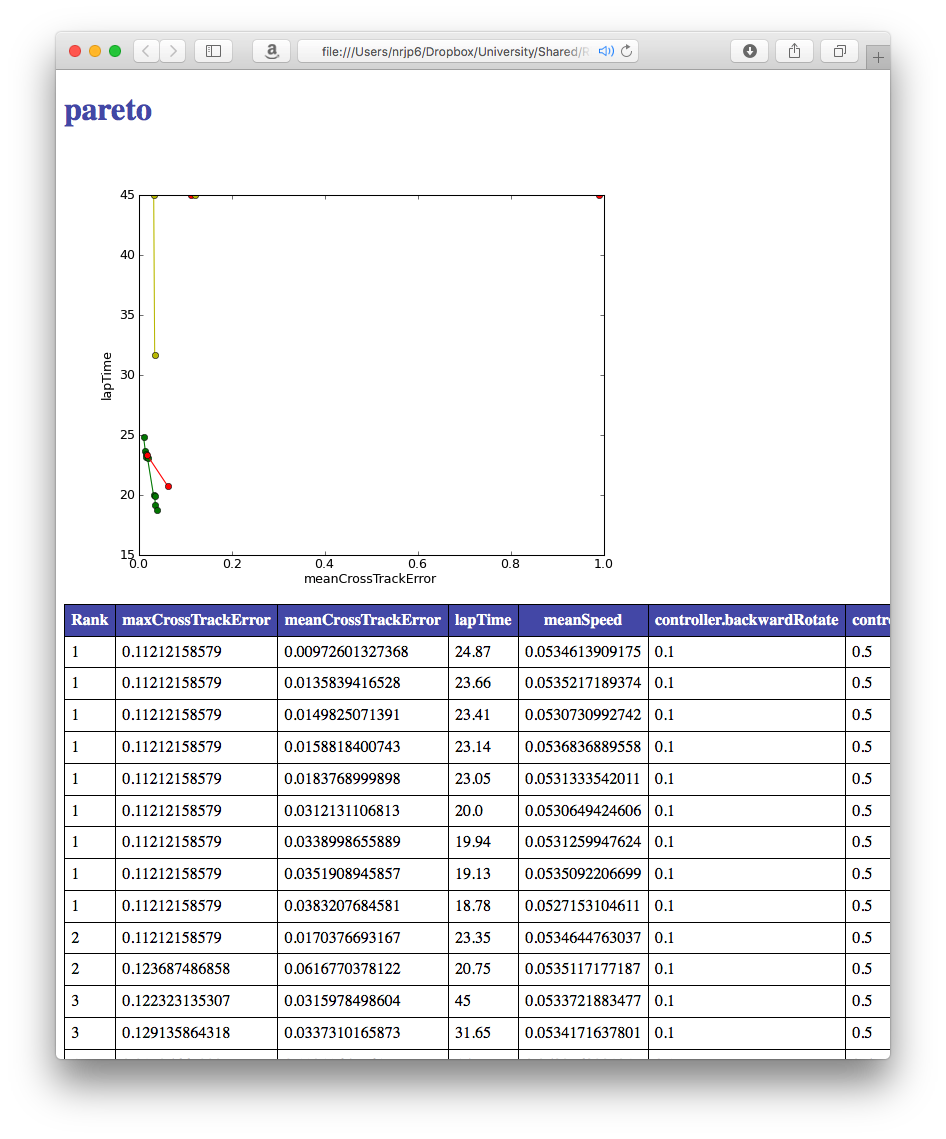
\includegraphics[width=0.9\textwidth]{figures/dse_results}
	\caption{DSE results}
	\label{fig:dse-results}
\end{figure}

\paragraph{An Approach to Effective DSE}
\label{sec:dse-algorithms}

Given a ``designed'' design space using the method detailed above, we use the INTO-CPS Tool Chain to simulate each design alternative. Whilst this approach is acceptable on small-scale studies, it quickly becomes infeasible as the design space grows. Inspired by processes found in nature, genetic algorithms ``breed'' new generations of optimal CPS designs from the previous generation's best candidates. This mimics the concept of survival of the fittest in Darwinian evolution.
Figure~\ref{fig:ga_dse_process} outlines the structure of a genetic algorithm used for DSE.  Several activities are reused from exhaustive DSE: simulation; evaluation of objectives; rank simulated designs; and generate results. The remaining activities are specific to the genetic approach and are detailed in the Methods Guidelines~\cite{INTOCPSD3.3a}.

\begin{figure}[h!]
	\centering
	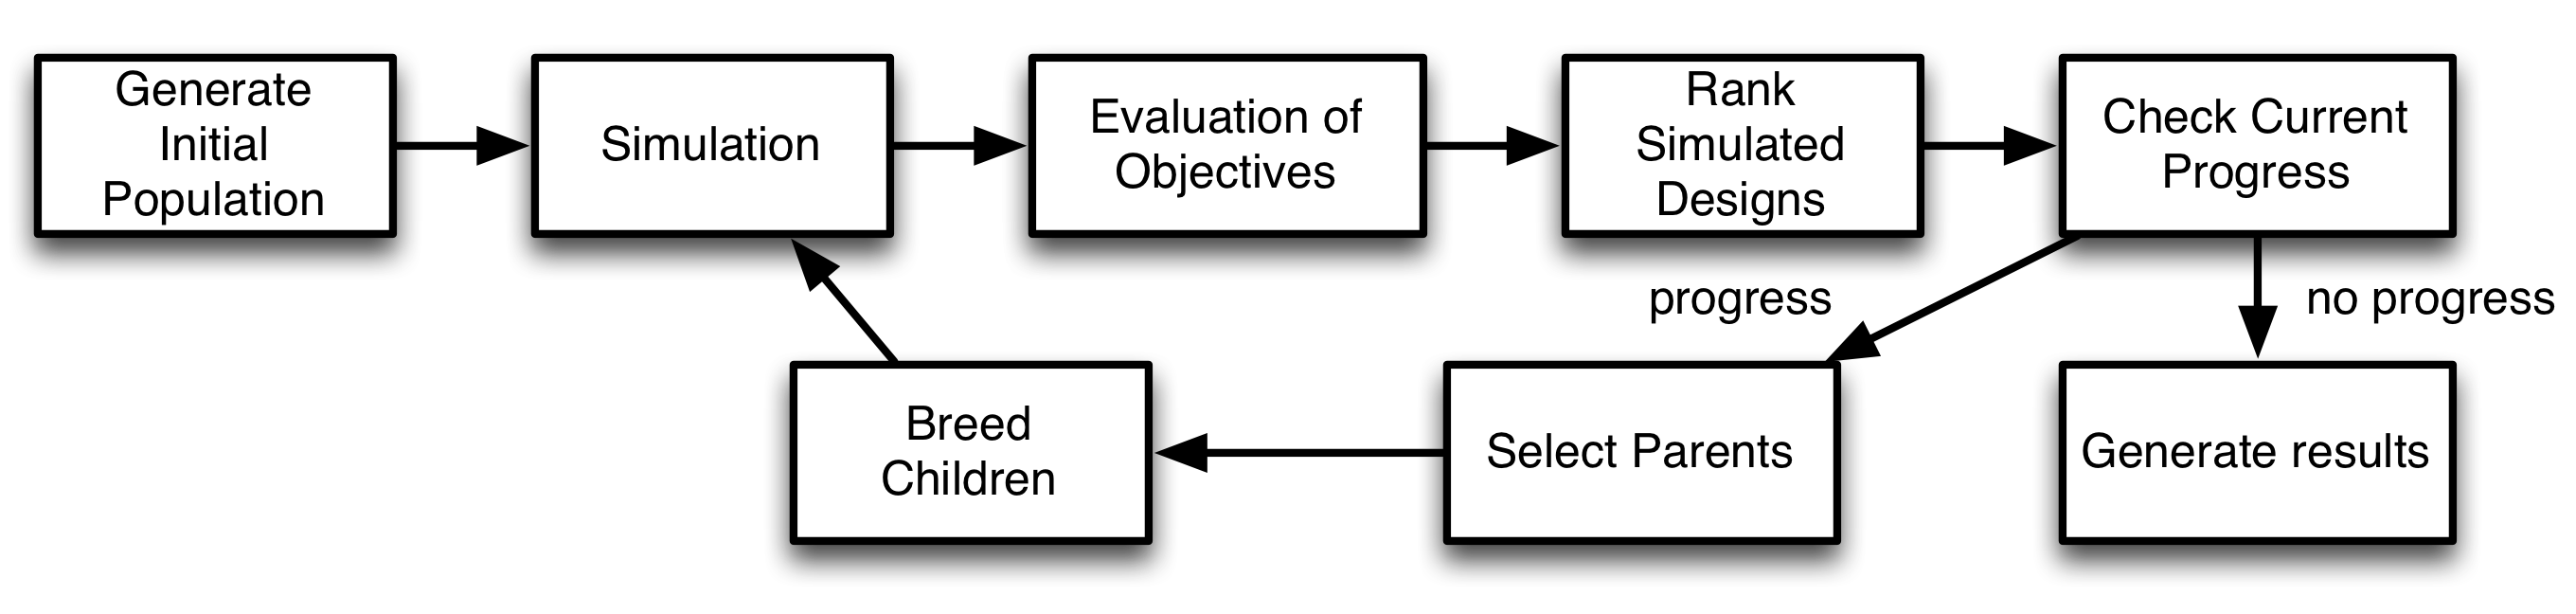
\includegraphics[width=0.9\textwidth]{figures/ga_process}
	\caption{High-level process for DSE Genetic Algorithm}
	\label{fig:ga_dse_process}
\end{figure}


An alternative to the genetic search, which is automated, is to use repeated exhaustive searches to home in on better regions of the design space.  In this approach the user would plan to perform multiple DSE experiments, each using some portion of their total simulation budget.  The first DSE experiment is used to cover the whole range of the design space, but not including all values for each parameter.   In this way the first DSE is used to locate regions of interest within the design space.  The regions of interest are areas of the design space that produced the better designs according to the ranking results, with the bounds of the 'area' defined by the parameter values that produced good results. The user then divides up their remaining simulation budget between the one or more areas of interest and perform further DSE on those areas.  
